\section{Heuristics}\label{heuristics}
The state evaluation function implemented for the minimax algorithm searches 
through each end-state, looking for instances of board-states that are known  
to affect the outcome of the match.
Our heuristic function is set, arbitrarily, to return a value [-100, 100], 
where a higher number means a higher valued state.

We have implemented three distinct intermediate state evaluation heuristics
and two final state evaluators. The intermediate state evaluators try to assign
a value to a state telling us how good or bad that state is if we would end up
in that state. The final state evaluators evaluates the final board state telling
us if there is a winning player or if the players tied.

\subsection{Wins}\label{win}
\begin{figure}[htb]
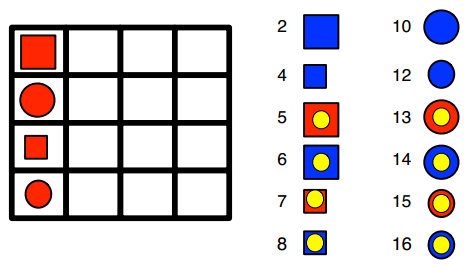
\includegraphics{pictures/win.png}
\caption[A \quarto{} win]{A winning board state in \quarto{}}
\label{fig:win}
\end{figure}
The most obvious board-state to look for is a win(see figure \ref{fig:win}), 
i.e. four pieces in a line  
sharing at least one attribute. To do this we compare all the pieces in each 
row, column and diagonal with each other and if a line is found where all 
pieces are equal we return a value of 100.

\subsection{Ties}
\begin{figure}[htb]
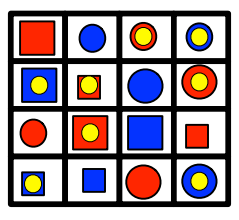
\includegraphics{pictures/tie.png}
\caption[A tie in \quarto{}]{A tied board state in \quarto{}}
\label{fig:tie}
\end{figure}
Another nice board-state to look out for is a tie(see figure \ref{fig:tie}), 
when all sixteen pieces have 
been placed on the board, but no win has been achieved. Checking this is merely 
counting if there are 16 pieces placed on the board, and if there is a  win. 
Since two optimal players will always tie\footnote{Proof of optimal play 
resulting in a tie: \url{http://web.archive.org/web/20041012023358/http://ssel.vub.ac.be/Members/LucGoossens/quarto/quartotext.htm}}, 
this is evaluated as 0, making sure that the minimax player will always 
choose a tie over a possible loss.

\subsection{Guaranteed losses}
\begin{figure}[htb]
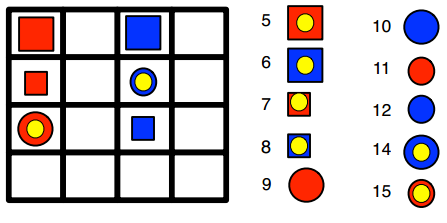
\includegraphics{pictures/gloss.png}
\caption[A guaranteed loss in \quarto{}]{A board state showing a guaranteed loss in \quarto{}}
\label{fig:gloss}
\end{figure}
When there are two distinct 3-piece lines which have opposite values of at least 
one attribute(see figure \ref{fig:gloss}), 
giving any piece to the opponent is a  guaranteed loss.
When we search for these states, we start of by finding all 3-piece lines on the 
board, then compare them to see if any of them have opposite values of an attribute.
Since a loss is the worst possible outcome of a game of \quarto{}, these states 
are valued at -100 in order to make the minimax player steer away from them.

\subsection{3-piece lines}
\begin{figure}[htb]
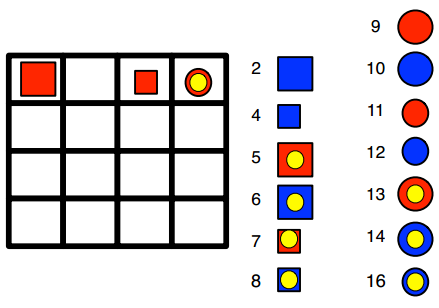
\includegraphics{pictures/3-odd.png}
\caption[A 3-piece line in \quarto{}]{A board state showing a 3-piece line with 
an odd number of winning pieces}
\label{fig:3-odd}
\end{figure}

\begin{figure}[htb]
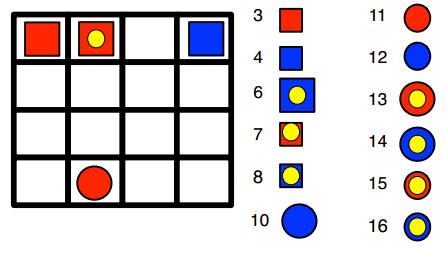
\includegraphics{pictures/3-even.png}
\caption[A 3-piece line in \quarto{}]{A board state showing a 3-piece line with 
an even number of winning pieces}
\label{fig:3-even}
\end{figure}
A board containing multiple 3-piece lines makes it difficult to give the 
opponent a non-winning piece to play. However, depending on whether there is 
an odd(see figure \ref{fig:3-odd}) or even(see figure \ref{fig:3-even}) 
number of pieces that can be placed in the final slot of a 
3-piece line, it is possible that the opponent will return a winning 
piece. With an even number of pieces the opponent can force us into giving
him a winning piece, and the other way around with and odd number of pieces. 
Since this is a risky strategy, the 3-piece lines with an even number 
of winning pieces are weighted heavier than the 3-piece lines with an odd 
number of winning pieces.

We have had a bit of debate around this last heuristic. Since it can be shown
that an optimal player always would tie the last heuristic can't force an opponent
into a losing situation, since the player could always finish off the line with
a non winning piece before being forced to give away a winning piece. For this
reason we were unsure whether or not the heuristics should be included or not.
In the end we included it because it should not hinder our performance, but
it can, against non optimal players, put us in a situation where we can win.

%TODO: include pictures
